\section{Experiments}
	\subsection{Data description}
		\subsubsection{BioHarness}
		From the data produced by the sensors more data can be derived. For the experiments the general log is used, because it has the most interesting variables and a lot preprocessing is already done. The heart rate is the amount of beats per minute and can be derived from the ECG. In the ECG graph (See Figure~\ref{fig:ecg}) a pattern is visible, also called a cycle. Each cycle is one heartbeat. 
			The accelerometer measures the acceleration magnitude. The peak acceleration is logged in the general log.
			The activity level is derived from the accelerometer and is expressed in terms of VMU\footnote{Vector Magnitude Units} (g).
			The force and directory of the gravity is known and the BioHarness is worn at the chest, so it's possible to calculate the posture of the user. The range is 180 degrees. \SI{0}{\celsius} is vertical and \SI{180}{\celsius} is inverted.
			Breath rate is derived from the breath sensor. The relative slow transfer rate from the device to the pc could be explained by the ?calculating/generation/computing? of the new data. The sampling frequency of the general log is \SI{1}{\hertz}.
		\subsubsection{Beddit}
		\label{sec:datadescriptionbeddit}
		The data from the sensors is being transferred via wifi or cable to the web servers from Beddit, almost realtime. The servers are analyzing the data and extracting the heart rate, respiration\footnote{Beddit is using the term respiration for breathing.} and the activity from the BCG. When all data is received of the night, the server is analyzing the data and will compute the sleep stages, sleep efficiency\footnote{Relative time sleeping compared to time in bed}, average heart rata, average noise level and stress level. The stages are "Away", "Wake", "Light sleep", "Deep sleep", "REM"\footnote{REM stands for Rapid Eye movements, it's a very light sleep and dreaming is possible in this stage.} and "Missing". Beddit doesn't use a constant sampling frequency. For the respiration and the instant heart rate there is a record for every beat, with the BPM computed from two single heart beats and the timestamp in seconds since the start of the session. Presence has a record for every second the presence is changing and a 0 if the user is not in bed and a 1 if the user is in bed. The binary actigram has a record for every second there is a movement above a certain threshold. The minutely actigram has for every minute a value with the amount of movements occurred. The temperature, ambient noise level and brightness have a record every 5 minutes with the date and time in ISO 8601\footnote{Example 2013-05-14T19:04\cite{iso8601}} format in locale time and their values, respectively celsius, decibel and lux.

		\subsubsection{OpenBeacon}
			The Openbeacon produces JSON and is stored in a NoSQL\footnote{A NoSQL database is the counterpart of a relational database. One argument to use it is because it's more flexible.} database MongoDB. The collections of the database can be exported as csv files.
			There are two collections. The collection tags, within documents with the format tag ID, timestamp\footnote{Amount of seconds since 00:00:00 GMT January 1, 1970 (the UNIX epoch)} . For every second the OpenBeacon sees a tag, a document will be added.
			The second collection is edges. For every second the OpenBeacon sees and edge between two tags, there will be one document added with the format ID of tag 1, ID of tag 2, power level and timestamp.
			The higher the power level the closer the tags are. The power level can not be expressed in terms of distance, because other things could interfere the power level. For example walls and other communication on the \SI{2.4}{\giga\hertz} frequency.
	\subsection{Beddit versus BioHarness}
		\subsubsection{Comparison}
			The first experiment is a comparison between the Beddit and the BioHarness. It's a good assignment to get go know the devices and the data. The two devices have overlapping features like the heart rate, breath rate and activity level. It would be a good test to see if they measure the same thing. 
			Beddit does not have a constant sampling frequency. After every heart beat the bpm is computed between the heartbeat and the previous heartbeat. The value is notated with the amount of seconds since the session. For every heartbeat, the associated minute and the heart rate is summed up with all the other heartbeat heart rates, and divided by the amount of heartbeats in that specific minute. This results in an average heart rate per minute. The respiration rate is also summed up, but doesn't needs to be divided, because it's the amount of breaths taken.
			The BioHarness heart rate, breath rate and activity calculations are done the same. The difference is that the Bioharness has a constant sampling frequency from \SI{1}{\hertz}. 
			The Beddit binary actigram has already one record per minute, it's just needs to be copied. It's not the same as the BiorHharness Activity, so it would be good to standardize\footnote{Standardization makes it easier to compare} the BioHarness activity and the Beddit binary actigram.
			\begin{figure}[h]
				\begin{equation}
					\label{eq:standardize}
					\mu = \frac{ \sum\limits_{i=1}^n y_i } { n }
				\end{equation}
				\begin{equation}
					D_i = (X_i - \mu)^2
				\end{equation}
				\begin{equation}
					\sigma = \sqrt{ \frac{ \sum\limits_{i=1}^n D_i } { n } }
				\end{equation}
				\begin{equation}
					standardized\ value_i = \frac{ y_i - \bar{y} } { \mu }
				\end{equation}
				\caption{Standardization method\cite{statistics}}
			\end{figure}

			Both devices were used for one night. The sampling frequency is \SI{16.67}{\milli\hertz} (every one minute). Minutes with missing data are removed. Section \ref{sec:datacollection} explains more about the setup and how to bundle the data. Sleeping with the BioHarness is possible when laying on the back. Sleeping on the left side is not comfortable. The tool QUICKIE\footnote{QUICKY stands for Quick User Interface for Convolution Kernel-Involving Experiments and is being made and used by the Data Minig Group of Liacs, but is not yet published.} is used to visualize the data and find the correlations.

		\subsubsection{Results}
			
			\begin{figure}[h]
				\centering
					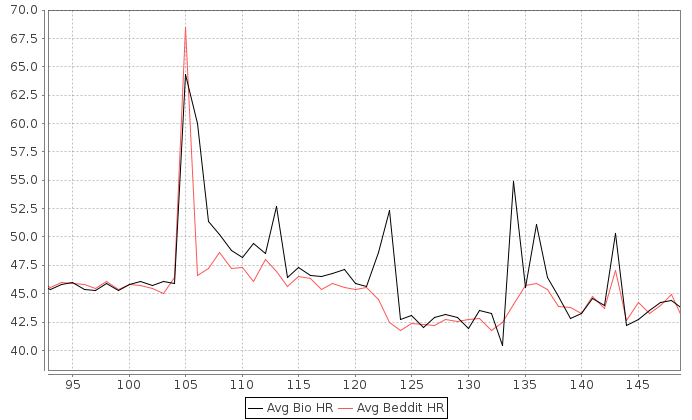
\includegraphics[scale=0.5]{avgbiovsavgbeddit.png}
					
				\caption{Part of the plot of the heart rate}
				\label{fig:avgbiovsavgbeddit}

			\end{figure}

			The lines in Figure~\ref{fig:avgbiovsavgbeddit} are not exactly the same, but have the same pattern. The correlation is 0.61. The low correlation could be explained by lag in measurements or one (or both) devices doesn't measure it correct. Moving average is a technique to smooth the lines. If width 7 is used, then it means a value on the new line is composed from the previous 3 minutes untill the next 3 minutes of the old line. With the heart rate example it will result in correlation of 0.98.\
						
			\begin{figure}[h]
				\centering
					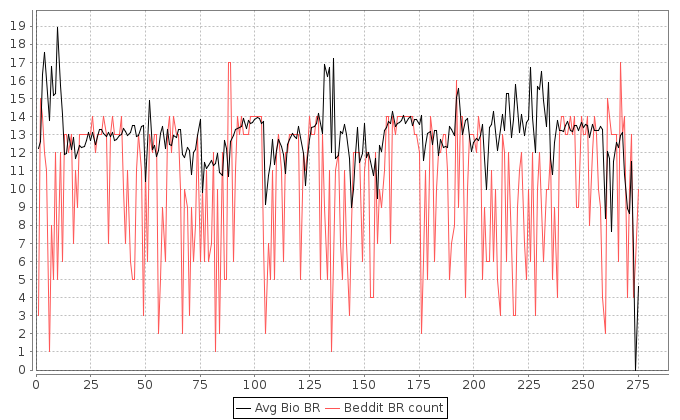
\includegraphics[scale=0.5]{vsbr.png}
					
				\caption{Plot of the breath rate}
				\label{fig:vsbr}

			\end{figure}

			The lines in Figure~\ref{fig:vsbr} are different. The correlation is 0.12, and even with moving average (width 10) used the correlation is still 0.47. There is something wrong, or the devices are measuring something else. The correlation of the standardized values is still 0.12. 
						
			\begin{figure}[h]
				\centering
					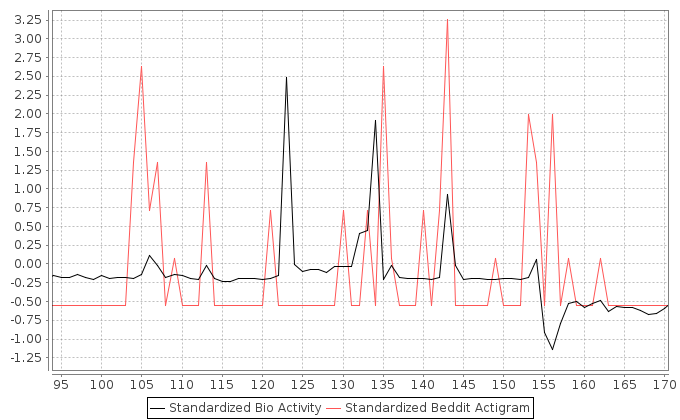
\includegraphics[scale=0.5]{vsactivity.png}
					
				\caption{Part of the plot of the activity}
				\label{fig:vsactivity}

			\end{figure}
			The Beddit actigram and the BioHarness activity are something different, so standardization is used. Figure~\ref{fig:vsactivity} shows some similarities, but the correlation is still low (0.26). Moving average doesn't help. 

			The heart rates of the Bioharness and the Beddit could be merged to one variable. The BioHarness breath rate and the Beddit respiration rate is totally different. The lines of the activity are a bit like each other, but the correlation of the activity is low and by far not good enough to merge it into one variable.

	\subsection{Data collection}
		\label{sec:datacollection}
		\paragraph{Beddit}
			The sensor is placed on my bed and connected with the device. The device is connected to the internet. Beddit starts measuring from 21:30 till 11:00 the next day. After all the measuring I've download for every night two JSON files with the API of Beddit\cite{bedditapi}. After the computing of the data I receive an e-mail and I visited the website to see if everything is logged alright.
		\paragraph{BioHarness}
			When I wake up, I start my PC and the BioHarness Log Downloader. After about 40 minutes I've took a shower and had breakfast, the Log Downloader is ready. I put the strap on my chest with the device and turn it on. After sport I take a shower and put it off and after shower again on. The device is water resistance up to one meter, but it takes a while for the strap to get dry. Right before I go to bed I connect the device to the PC so it's recharged again the next day. I'm missing a few minutes data every day because of the Log Downloader and the showering. 
		\paragraph{Openbeacon}
			In the experiment the OpenBeacon is used as a localization tool. The location of the user could explain some behaviour during the day, which can explain behaviour during the night. At first there were two OpenBeacon devices available, one for the ground floor and one for the second floor. It covered the whole house, but unfortunately one device stopped working. The working device were set up at the ground floor and several tags at the following places: dining room, toilet ground floor, kitchen, living room, hall first floor, toilet first floor. I were wearing also a tag. If there was an edge between my tag and the tag dining room, my location was the dining room etc. The OpenBeacon was always on, but the script to capture the JSON output and storage it in the MongoDB not. After waking up I started my laptop and the script. I took my tag with me, except in the shower where it was put at on a cabinet at the hall first floor. When I left the house the script was turned off and when I came back home I turned the script on right away. There's a few minutes missing data every day. For example, I'm late back home from sport and I went to bed, but not before changing clothes, brushing teeth, unpacking my sport bag etc, without wearing my tag, because the script was not running. Of course the script turned off before going to bed.

			
			A few locations were I was at a certain time are known, but we can extract more locations with some tricks. See Figure~\ref{fig:decisiontree} for the decision tree.

				\begin{figure}[h!]
					\begin{tikzpicture}[
% Gates and symbols style
    and/.style={and gate US,thick,draw,fill=red!60,rotate=90,
		anchor=east,xshift=-1mm},
    or/.style={or gate US,thick,draw,fill=blue!60,rotate=90,
		anchor=east,xshift=-1mm},
    be/.style={circle,thick,draw,fill=green!60,anchor=north,
		minimum width=0.7cm},
    tr/.style={buffer gate US,thick,draw,fill=purple!60,rotate=90,
		anchor=east,minimum width=0.8cm},
% Label style
    label distance=3mm,
    every label/.style={blue},
% Event style
    event/.style={rectangle,thick,draw,fill=yellow!20,text width=2cm,
		text centered,font=\sffamily,anchor=north},
% Children and edges style
    edge from parent/.style={very thick,draw=black!70},
    edge from parent path={(\tikzparentnode.south) -- ++(0,-1.05cm)
			-| (\tikzchildnode.north)},
    level 1/.style={sibling distance=7cm,level distance=1.4cm,
			growth parent anchor=south,nodes=event},
    level 2/.style={sibling distance=7cm},
    level 3/.style={sibling distance=6cm},
    level 4/.style={sibling distance=3cm}
%%  For compatability with PGF CVS add the absolute option:
%   absolute
    ]
%% Draw events and edges
    \node (g1) [event] {No flow to receiver}
	     child{node (g2) {No flow from Component B}   
	     	child {node (g3) {No flow into Component B}
	     	   child {node (g4) {No flow from Component A1}
	     	      child {node (t1) {No flow from source1}}
	     	      child {node (b2) {Component A1 blocks flow}}
			}
	     	   child {node (g5) {No flow from Component A2}
	     	      child {node (t2) {No flow from source2}}
	     	      child {node (b3) {Component A2 blocks flow}}
			}
		   }
	     	child {node (b1) {Component B blocks flow}}
		};
%% Place gates and other symbols
%% In the CVS version of PGF labels are placed differently than in PGF 2.0
%% To render them correctly replace '-20' with 'right' and add the 'absolute'
%% option to the tikzpicture environment. The absolute option makes the 
%% node labels ignore the rotation of the parent node. 
   \node [or]	at (g2.south)	[label=-20:G02]	{};
   \node [and]	at (g3.south)	[label=-20:G03]	{};
   \node [or]	at (g4.south)	[label=-20:G04]	{};
   \node [or]	at (g5.south)	[label=-20:G05]	{};
   \node [be]	at (b1.south)	[label=below:B01]	{};
   \node [be]	at (b2.south)	[label=below:B02]	{};
   \node [be]	at (b3.south)	[label=below:B03]	{};
   \node [tr]	at (t1.south)	[label=below:T01]	{};
   \node [tr]	at (t2.south)	[label=below:T02]	{};
%% Draw system flow diagram
   \begin{scope}[xshift=-7.5cm,yshift=-5cm,very thick,
		node distance=1.6cm,on grid,>=stealth',
		block/.style={rectangle,draw,fill=cyan!20},
		comp/.style={circle,draw,fill=orange!40}]
   \node [block] (re)					{Receiver};
   \node [comp]	 (cb)	[above=of re]			{B}  edge [->] (re);
   \node [comp]	 (ca1)	[above=of cb,xshift=-0.8cm]	{A1} edge [->] (cb);
   \node [comp]	 (ca2)	[right=of ca1]			{A2} edge [->] (cb);
   \node [block] (s1)	[above=of ca1]		{Source1} edge [->] (ca1);
   \node [block] (s2)	[right=of s1]		{Source2} edge [->] (ca2);
   \end{scope}
\end{tikzpicture}

					\caption{A decision tree how to find more locations}
					\label{fig:decisiontree}
				\end{figure}

				Strange enough some tags showed up which were not part of the tags from the OpenBeacon. These 'tags' were ignored.
				
	\subsection{Preprocessing}
		\subsubsection{From raw to a dataset}
			In this phase all the data is used and combined to have one structed dataset after the fase. The end result is a csv file. The sampling frequency is \SI{1}{\hertz}, which means for every second a row. The dataset begins at Wed 10 Apr 2013 08:43:01 AM CEST GMT+2 and ends at Thu 25 Apr 2013 08:52:35 AM CEST GMT+2. 
			
			%\pagebreak

\lstset{
	language=Python,
	numbers=left,
	numberstyle=\tiny,
	frame=tb,
	basicstyle=\small,
	tabsize=2,
}
\begin{lstlisting}[caption=Pseudocode]
// Initializing
data = []
begin = 10 April 2013 08:43:01
end = 25 April 2013 08:52:35
for every second from begin to end:
	data[second] = {}

// Reading
for every day:
	// Beddit
	beddit = readBedditFiles(day)
	for 'presence', 'respiration', 'ihr', 'sleep stage', 'noise',
		'luminosity', 'temperature', 'minutely actigram' as attribute:
		for every attribute in beddit as value:
			timestamp = convertToTimestamp(value)
			data[timestamp]['beddit' + attribute] = value

	?OR?

	for every presence in beddit:
		timestamp = convertTime(presence)
		data[timestamp]['beddit'] = presense
	for every respiration in beddit:
		timestamp = convertTime(respiration)
		// Amplitude, minToMin, maxToMax
		data[timestamp]['beddit_respiration'] = respiration
	for every ihr in beddit:
		timestamp = convertTime(ihr)
		// Instant heart rate
		data[timestamp]['beddit_ihr'] = ihr
	for every sleep stage in bddit:
		timestamp = convertToTimestamp(sleep stage)
		data[timestamp]['beddit sleep stage'] = sleep stage

	// BioHarness
	bioharness = readBioharnessFile(day)
	timestamp = getTime(bioharness)
	for every second in bioharness:
		for 'hr', 'br', 'activity', 'acceleration', 'posture',
			'BRAmplitude', 'ECGAmplitude', 'ECGNoise', 'XMin', 'XPeak',
			'YMin', 'YPeak', 'ZMin', 'ZPeak' as attribute:
			data[timestamp]['bioharness ' + attribute] = second[attribute]


	// OpenBeacon
		// set all locations 0
		for every second of the day
			for 'out', 'dining room', 'toilet ground floor', 'kitchen',
				'living room', 'toilet first floor', 'rest', 'bed' as location:
				data[timestamp][location] = 0

		openbeacon = readerOpenBeaconFile(day)
		for every second in openbeacon:
			timestamp = getTimestamp(second)
			// See Figure Decision Tree
			location = findLocation(openbeacon, data[timestamp])
			data[timestamp][location] = 1

// Writing csv file

writeHeader()
for every second in data:
	row = []

	// Copy OpenBeacon
	for 'out', 'dining room', 'toilet ground floor', 'kitchen',
		'living room', 'toilet first floor', 'rest', 'bed' as location:
		row[location] = data[second][location]

	// Copy Beddit respiration
	for 'amplitude', 'minToMin', 'maxToMax' as attribute:
		if 'beddit respiration ' + attribute in data[second]:
			row['beddit respiration ' + attribute] = 
				data[second]['beddit ' + attribute]
		else:
			row['beddit respiration ' + attribute] = 'null'

	// Copy rest of Beddit
	for 'ihr', 'sleep stage', 'noise', 'luminosity', 'temperature',
		'minutely actigram' as attribute:
		if 'beddit ' + attribute in data[second]:
			row['beddit ' + attribute in data[second] =
				data[second]['beddit ' + attribute]
		else:
			row['beddit ' + attribute in data[second] = 'null'

	// Copy BioHarness
	for 'hr', 'br', 'activity', 'acceleration', 'posture',
			'BRAmplitude', 'ECGAmplitude', 'ECGNoise', 'XMin', 'XPeak',
			'YMin', 'YPeak', 'ZMin', 'ZPeak' as attribute:
		if 'bioharness ' + attribute in data[second]:
			row['bioharness ' + attribute =
				data[second]['bioharness ' + attribute]
		else
			row['bioharness ' + attribute = 'null'

	// Write row
	writeRow(row)

	

\end{lstlisting}


			Most of the code is loops and loops, calculating the right timestamp and copy data. 
			The Beddit API only give records of the sleep stage and timestamp, when the stage is changing.
			In the csv file the gap is filled in with missing values. There are still a lot of missing values. For example the heart rate at night. It is possible to use methods to fill in the gaps, but it's better to provide a 'raw' dataset, with only the facts. When someone would like to use the data, the person can decide herself/himself the method or solution.
			\begin{figure}[h!]
			\[ 
				\left(
				\begin{array}{c}
				Away \\
				null \\
				null \\
				Wake \\
				null \\
				Light sleep \\
				Deep sleep \\
				null \\
				Light sleep \\
				null \\
				Wake \\
				Away \\
				null
				\end{array}
				\right)
				\to
				\left(
				\begin{array}{c}
				Away \\
				Away \\
				Away \\
				Wake \\
				Wake \\
				Light sleep \\
				Deep sleep \\
				Deep sleep \\
				Light sleep \\
				Light sleep \\
				Wake \\
				Away \\
				Away 
				\end{array}
				\right)
			\] 
			\caption{How the missing values are filled in of the sleep stages}
		\end{figure}



			%Difficult because of the differnet devices has different frequenties, different data format/extraction. 
			%Dataset, every second from start till end is a row. BioHarness already gives an 1Hz dataset, so fill in the values if BioHarness is on. 
			%Openbeacon is 4Hz and can easily converted to 1Hz.
			%Beddit is difficult, some attributes are received once per 5 minutes and some attributes are between 4 and 15 seconds, not constant at all. Format of time sometimes seconds after interval\_start and sometime datetime.
		\subsubsection{Extend the dataset}
			Example how to use fill in the gaps.
			filling the beddit heart rate gaps with interpolation.
			Merging the beddit heart rate with the BioHarness. 
			Still 15.96\% is missing. 
			Fill in the gaps again with interpolation
		
